\section{Introduction}
\label{sec:intro}

We are interested in the nonlinear response of a single-degree-of-freedom system under both \emph{periodic} and \emph{stochastic} external excitations. The general form of the equations studied here is given by

\begin{equation}
\ddot q_t + \frac{\partial U}{\partial q}(q_t) + G(q_t, \dot q_t) \dot q_t
= \mu_0 \cos(\omega t) + \mu_1 \xi(t),
\label{E:geom}
\end{equation}
where $q \in \reals$ represents a generalized coordinate and the potential $U: \reals \to \reals$ has a single well. More precisely, we require that $U \in C^\infty(\reals; \reals_+)$, that $\lim_{|x|\to\infty}U(x) = \infty$, that
\[
\{x \in \reals: U^\prime(x) = 0\} = \{x \in \reals: U(x)=0\} = 0,
\]
and that $\omega_0^2 \equiv U^{\prime \prime}(0)>0$. See Figure~\ref{F:Pot}.
\begin{figure}
\begin{equation*}
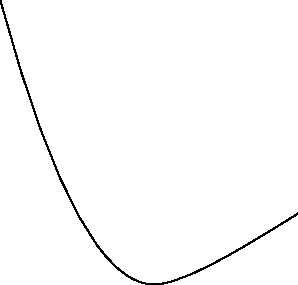
\includegraphics[width=\textwidth*1/3]{figures/pot}
\end{equation*}
\caption{Potential energy}
\label{F:Pot}
\end{figure}

In~\eqref{E:geom}, $G$ represents dissipative terms, and $\xi$ represents mean zero, stationary, independent Gaussian white noise processes. For convenience, we shall define
\[
U_h(q) \equiv U(q) + \frac12 \omega_0^2 q^2. \qquad q \in \reals
\]
Since an exact solution of~\eqref{E:geom} is not known, the purpose of the present analysis is to develop a stochastic averaging technique of perturbed two-dimensional Hamiltonian systems with an elliptic fixed point. The analytical methods presented are based on \citet{freidlin98:_random_pertur_nonlin_oscil, namachchivaya01:_unified_approac_noisy_nonlin_mathieu_type_system, namachchivaya02:_rigor_stoch_averag_center_addit_noise, sowers03:_stoch_averag_near_homoc_orbit}.

Introducing appropriate scaling of parameters for the nonlinear, dissipative, and time dependent terms, we recast~\eqref{E:geom} as
\begin{equation}
\ddot q_t^\epsilon + \omega_0^2 q_t^\epsilon + \epsilon^n \frac{\partial U_h}{\partial q}(q_t^\epsilon) + \epsilon^d G(q_t^\epsilon,\dot q_t^\epsilon) \dot q_t^\epsilon = \epsilon \mu_0 \cos(\omega t) + \epsilon^\nu \mu_1 \xi(t),
\label{E:geom_scale}
\end{equation}
Our interest is the behavior of $q$ in a certain \emph{limiting regime}. Depending on the values of $n,d,\nu$, the limiting dynamics of the state $(q^\epsilon,\dot q^\epsilon)$ as $\epsilon \to 0$ are significantly different. In \citet{namachchivaya01:_unified_approac_noisy_nonlin_mathieu_type_system} a unified approach for noisy weakly nonlinear systems like~\eqref{E:geom_scale} was developed for the case when $n=1$. Here, by appropriate scaling of the nonlinear term $\partial U_h/\partial q$, the solution $(q^\epsilon,\dot q^\epsilon)$ over any finite interval converges in probability, as $\epsilon \to 0$, to the solution of an averaged equation which has a conservation law. The averaged equation has certain nontrivial (yet generic) types of fixed points. The evolution of the first integral (associated with a conservation law) was examined on a rescaled time interval.

A number of researchers have worked on Duffing oscillators in various environments. In the absence of noisy perturbations (i.e., $\mu_1=0$), equation~\eqref{E:geom_scale} represents a harmonically forced nonlinear oscillator. This has been studied extensively \citep{guckenheimer83:_nonlin, nayfeh79:_nonlin_oscil}. On the other hand, in the absence of periodic perturbations (i.e., $\mu_0 = 0$),~\eqref{E:geom_scale} represents the noisy \emph{Duffing-van der Pol} equation which has been studied by \citet{arnold96:_towar_hopf, liang99:_stoch_dynam, lin67:_probab_theor_struc_dynam} and \citet{bolotin84:_random}, to name a few. Here the work of \citet{namachchivaya01:_unified_approac_noisy_nonlin_mathieu_type_system} is extended to include more general (strongly) nonlinear systems ($n=0$ in~\eqref{E:geom_scale}) and obtain analytical results for a low-dimensional model of~\eqref{E:geom_scale}. \emph{Stochastic averaging} can achieve model-reduction for two different sets of values of $d$ and $\nu$. Here, we consider the case in which the order of the noise equals that of the dissipation, i.e., $d = \nu = 1$. Note that when the noise intensity is larger than the dissipative or periodic perturbations, i.e., $\nu=1/2$, it becomes possible to use the results of \citet{pinsky88:_lyapun}. Pinsky-Wihstutz scaling stretches the coordinates in such a way that to leading order, stochastic forcing induced diffusion balances dissipative drift.

It is well known that stochastic resonance (SR) can arise in under-damped systems with a single-well potential, unlike \emph{conventional} SR in multi-well potentials. Therefore, to study such SR, we shall consider a prototypical single-well potential
\[
U(q) = \frac12 q^2 + \frac14 q^4 + Bq
\]
with two distinct cases depending on the constant $|B|$. In the first case, when $|B| \le B_c$ the nonlinear oscillation frequency $\Omega(E)$ monotonically increases with total energy $E$ as shown in Figure~\ref{F:frequency}(a). In the second case with $|B| > B_c$, the system frequency $\Omega(E)$ is non-monotonic as sketched in Figure~\ref{F:frequency}(b). Furthermore, in the absence of the periodic forcing, the under-damped oscillator exhibits the so-called sharp \emph{zero-dispersion spectral peaks} (ZDPs) close to the extremal frequency $\Omega_m$ in the fluctuation spectrum. The magnitude of the ZDP climbs up exponentially with increasing noise strength $\mu_1$. The extreme narrowness of the ZDP~\citet{soskin89:_fluct, soskin92:_evolut} suggests that stochastic resonance in the latter case is far more dramatic phenomenon than in the former case. Here, we investigate the system with a symmetric single potential, i.e., $B=0$ and the constant damping coefficient, $G(q^\epsilon_t,\dot q_t^\epsilon) = \zeta$. Thus Equation~\eqref{E:geom_scale} becomes
\[
\ddot q_t^\epsilon + \epsilon \zeta \dot q_t^\epsilon + q_t^\epsilon + {q_t^\epsilon}^3 = \epsilon \mu_0 \cos (\omega t) + \epsilon \mu_1 \xi(t)
\]

In section~\ref{S:problem setup} is devoted to setting up a framework to study the effect of random perturbation of the system near the resonance surface. In other words, adequately scaled local coordinates adjacent to the resonance surface are introduced from the system in action space. In section~\ref{S:reduction}, a cascaded averaging approach is presented for the local system under the capture into resonance. More specifically, we address a separation of time scales so that state variables of fast time scale can be averaged out while the equation of the slow variable is approximated. The near resonant motion is reduced to a graph valued process which turns out to converge weakly to a Markov process with a limiting generator. Section~\ref{S:stationary pdf} presents stationary probability density from the limiting generator which characterize the reduced Markov process. In the final section, we give conclusion and conjecture regarding the effect of SR.

\section{Problem Setting}
\label{S:problem setup}

By making use of the system Hamiltonian with strong nonlinear terms, we write~\eqref{E:geom} with the standard rescaling for dissipation, as a weakly perturbed Hamiltonian system
\begin{equation}
\begin{aligned}
\dot x_t^\epsilon &= \frac{\partial {\mathcal H}(x_t^\epsilon,y_t^\epsilon)}{\partial y}\\
\dot y_t^\epsilon &= -\frac{\partial {\mathcal H}(x_t^\epsilon,y_t^\epsilon)}{\partial x} + \epsilon F^y (x_t^\epsilon, y_t^\epsilon, \theta_t) + \epsilon G^y(x_t^\epsilon, y_t^\epsilon) \xi(t)\\
\dot \theta_t &= \omega,
\end{aligned}
\label{E:eom-qp-eps}
\end{equation}
where $(x_0^\epsilon, y_0^\epsilon)\equiv(x,y) \in \reals^2$, $\theta_0 \equiv \theta \in S$. The unperturbed ($\epsilon = 0$) equations corresponding to~\eqref{E:eom-qp-eps} form a Hamiltonian
\[
\mathcal H (x,y) = \frac{y^2}{2} + U (x)
\]
where $U(x) = x^2/2+x^4/4$. We apply a canonical transformation to obtain new variables $\phi, I$ in such a way that the transformed Hamiltonian remains a constant, $I$, and the angle $\phi$ increases by one during every period of rotation. The conjugate momentum corresponding to $\phi$ is the action $I$. Thus, the unperturbed integrable Hamiltonian equations with elliptic fixed points can be written as
\begin{align}
\dot I_t &= 0, & \dot \phi_t &= \Omega (I_t), & \dot \theta_t &= \omega,
\label{E:eom-aca-zero}
\end{align}
and the perturbed equations \eqref{E:eom-qp-eps} simplify to the following Stratonovich equations
\begin{equation}\begin{aligned}
d I_t^\epsilon &= \epsilon f^I(I_t^\epsilon, \phi_t^\epsilon, \theta_t) dt + \epsilon g^I (I_t^\epsilon, \phi_t^\epsilon) \circ dW_t\\
d \phi_t^\epsilon &= \Omega(I_t^\epsilon) dt + \epsilon f^\phi (I_t^\epsilon, \phi_t^\epsilon, \theta_t) dt+ \epsilon g^\phi (I_t^\epsilon, \phi_t^\epsilon) \circ dW_t\\
d \theta_t &= \omega d t,
\end{aligned}\label{E:eom-aca-eps}
\end{equation}
where $I_0=I \in \reals, \phi_0 = \phi \in S, \theta_0=\theta \in S$. $S$ denotes the circle with unit radius in 2-dimensional Euclidean space. We shall use the dominant global dynamics and the \emph{phase-space stratification} of~\eqref{E:eom-aca-zero} to capture the long-term behavior of the dissipative, periodically driven, noisy system~\eqref{E:eom-aca-eps}.

As stated in the introduction, our principal technique of dimensional reduction will be the method of stochastic averaging for nonlinear systems with small noise. As the noise becomes asymptotically small, one can exploit separation of scales to find an appropriate lower-dimensional description of the system for many important random vibration problems. The unique feature in our treatment will be the inclusion of resonances, as we shall describe below.

\subsection{Resonances in Two Frequency System}

In an integrable Hamiltonian system such as~\eqref{E:eom-aca-zero}, if the frequencies are non-commensurable, then the orbits are everywhere dense on $S^2$ and the motion corresponding to the unperturbed system~\eqref{E:eom-aca-zero} is called \emph{quasi-periodic}. Resonance occurs when the frequencies are commensurable or nearly commensurable, and the closure of an orbit is a one-dimensional torus. Since $\Omega$ depends on the action $I$, the resonance will depend on certain values of the action.

\begin{definition}[Resonance]
For the two-phase system, resonances occur when $\Omega$'s, are connected by a commensurability relation
\begin{align}
\kappa_1 \,\Omega(I) + \kappa_2 \, \omega &= 0, & \kappa &= (\kappa_1,\kappa_2) \in \integers^2 - (0,0)
\label{E:resonance}
\end{align}
and the order of the resonance is given by $|\kappa| = \sum_{i=1}^2 \kappa_i$.
\end{definition}
If we regard $(\kappa_1,\kappa_2) \in \integers^2 -(0,0)$ as fixed, then~\eqref{E:resonance} is a single equation in one unknown. Away from the equilibrium point~($\Omega(I) \neq 0$) and at a particular value $I^{m:n}$ with $(\kappa_1,\kappa_2)=(m,-n)$, we have
\[
\frac{\Omega(I^{m:n})}{\omega} = \frac{n}{m} \in \rationals
\]
So each rational value assumed by the above frequency ratio corresponds with a resonance domain, in principal, an infinite number of such resonance domains exist.
\begin{definition}[Resonance Module: $\Omega^{\perp}$]
For some fixed $I$, the resonance module is a 2-dimensional integer vector
\[
\Omega^{\perp} \equiv \{ \kappa = (\kappa_1,\kappa_2) \in \integers^2 - (0,0): \kappa_1 \Omega(I) + \kappa_2 \omega = 0 \}
\]
\end{definition}
\begin{definition}[Resonance Set: $\reals_k$]
The resonance set are those values of $I$ for which a particular resonance $\kappa = (m,-n) \in \integers^2 - (0,0)$ occurs, i.e.,
\[
\reals_k \equiv \{ I \in \dom \subset \reals^2: \kappa_1 \Omega(I) + \kappa_2 \omega  = 0, \kappa = (\kappa_1,\kappa_2) \in \integers^2 - (0,0) \}
\]
\end{definition}
A resonance set is a point in the one-dimensional action space and this point along with the variables $(\phi, \theta) \in S^2$ forms, what is often called a resonance surface.
\begin{figure}[htbp]
\centering
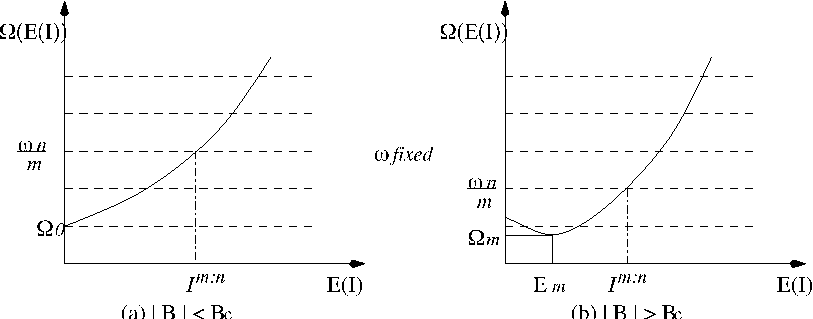
\includegraphics[width=\textwidth]{figures/freq}
\caption{Resonance sets for the Duffing equation}
\label{F:frequency}
\end{figure}
For some fixed $(\kappa_1,\kappa_2) = (m,-n)$, the resonance set for the Duffing equation, for example, consists of just one point $I^{m:n}$. When the trajectory of a phase point arrives at this surface, the trajectory either passes through the resonance and gets away from the resonant surface or gets captured into resonance. The captured trajectory moves slowly while preserving the resonance condition and may leave the resonance surface after a time interval of order $\epsilon^{-1}$. In the next section we describe the perturbed stochastic dynamics of system~\eqref{E:eom-qp-eps} close to this resonance surface with the aim of determining the effects of noisy perturbations on the passage of trajectories through the resonance zone.

\subsection{Scaling Close to a Resonant Surface}
\label{S:scaling}

The near resonant motion of randomly perturbed integrable systems is not well understood. In this section, we will study this problem in depth by introducing local coordinates close to the resonance surface. A point ($I,\phi,\theta$) in the neighborhood of the resonant surface will be specified by $r$, the distance to the resonant surface, and the angles ($\gamma,\theta$). Since in the frequency plane, $\Omega(I)-\omega$, the resonance curve forms a straight line through the origin with the normal defined by $r \equiv m \Omega(I) - n \omega$. If we assume
\[
\frac{\partial \Omega}{\partial I} (I) \neq 0
\]
then the transformation is invertible, i.e. $I=I(r)$. Hence, we introduce a distance to the resonant manifold as
\[
\eta \equiv I - I^{m:n},
\]
Making use of~\eqref{E:eom-aca-zero} we introduce a slow angle $\gamma$
\[
m \dot \phi - n \dot \theta = \frac{d}{dt} \left(m \phi - n \theta \right) \equiv \frac{d \gamma}{dt}, \quad \text{for} \quad \kappa =(m,-n) \in \Omega^{\perp}.
\]
and it is clear that there is a 2$\times$2 matrix
\[
A = \left[
\begin{array}{cc} m & -n \\ 0 & 1 \\ \end{array} \right],
\]
with $m \neq 0$. The matrix $A$ satisfies $A \cdot \Omega = [0, \omega]^\text{T}$ and it can be used to transform between fast and slow variables since $A \cdot [\phi, \theta]^\text{T} = [\gamma, \theta]^\text{T}$. We can write the evolutions in the new variables $\eta_t^\epsilon,\gamma_t^\epsilon,\theta_t$ using the Taylor expansion, about $\eta = 0$ as
\begin{equation}
\begin{aligned}
d {\eta}_t^\epsilon &= \epsilon \left\{
f^I(I^{m:n},\phi_t^\epsilon(\gamma_t^\epsilon,\theta_t),\frac{\theta_t}{\omega}) + \frac{\partial f^I}{\partial I}(I^{m:n},\phi_t^\epsilon(\gamma_t^\epsilon,\theta_t),\frac{\theta_t}{\omega}) \, {\eta}_t^\epsilon \right.\\
&\quad \left. + \frac12 \frac{\partial ^2 f^I}{\partial I ^2}(I^{m:n},\phi_t^\epsilon(\gamma_t^\epsilon,\theta_t),\frac{\theta_t}{\omega}) \, ({\eta}_t^\epsilon)^2 \right\} + \epsilon \left\{g^I(I^{m:n}, \phi_t^\epsilon(\gamma_t^\epsilon, \theta_t)) \right.\\
&\quad \left. + \frac{\partial g^I}{\partial
I}(I^{m:n},\phi_t^\epsilon(\gamma_t^\epsilon,\theta_t)) \,
{\eta}_t^\epsilon + \frac12 \frac{\partial^2 g^I}{\partial I^2}(I^{m:n},\phi_t^\epsilon(\gamma_t^\epsilon,\theta_t)) \, ({\eta}_t^\epsilon)^2\right\} \circ dW_t\\
d {\gamma}_t^\epsilon &= m \frac{\partial \Omega}{\partial I}
(I^{m:n}) {\eta}_t^\epsilon +\frac{m}{2}\frac{\partial
^2\Omega}{\partial I^2} (I^{m:n}) ({\eta}_t^\epsilon)^2
 + \epsilon  m \left\{ f^{\phi}(I^{m:n},\phi_t^\epsilon(\gamma_t^\epsilon,\theta_t),\frac{\theta_t}{\omega}) \right.\\
&\quad + \left.\frac{\partial f^{\phi}}{\partial
I}(I^{m:n},\phi_t^\epsilon(\gamma_t^\epsilon,\theta_t),\frac{\theta_t}{\omega})
\, {\eta}_t^\epsilon+ \frac12 \frac{\partial^2 f^{\phi}}{\partial
I^2}(I^{m:n},\phi_t^\epsilon(\gamma_t^\epsilon,\theta_t),\frac{\theta_t}{\omega})
({\eta}_t^\epsilon)^2\right\}\\
&\quad + \epsilon m \left\{g^{\phi}(I^{m:n},\phi_t^\epsilon(\gamma_t^\epsilon,\theta_t))
+ \frac{\partial g^{\phi}}{\partial
I}(I^{m:n},\phi_t^\epsilon(\gamma_t^\epsilon,\theta_t)) \eta_t^\epsilon\right.\\
&\quad + \left.\frac12 \frac{\partial^2 g^{\phi}}{\partial I^2}(I^{m:n},\phi_t^\epsilon(\gamma_t^\epsilon,\theta_t)) ({\eta}_t^\epsilon)^2\right\} \circ dW_t\\
d {\theta}_t &= \omega d t \quad \text{where} \quad
\phi_t^\epsilon(\gamma_t^\epsilon,\theta_t)\equiv\frac{\gamma_t^\epsilon}{m}+\frac{n}{m}\theta_t
\end{aligned}
\label{E:pw}
\end{equation}
On the resonant surface $\eta=0$ and in the neighborhood of that surface $\eta$ is small, since the effect of a resonance is felt in a narrow strip about the resonance line called the \emph{resonant zone}. Due to the nilpotent structure of the zeroth order terms in equations~\eqref{E:pw}, we need an appropriate scaling to capture the dynamics in the proximity of the resonant zone. For the case of interest in the current analysis (i.e. noise intensity  of the same order as the dissipative perturbation) the width of the resonant zone is of order $\sqrt\epsilon a_k$ where $a_k$ is an upper bound for the amplitudes of the resonant harmonics of the perturbations. Accordingly, $\eta$ is rescaled:
\[
\eta = \epsilon^\frac12 h.
\]
Thus, we obtain the following set of stochastic equations from~\eqref{E:pw}
\begin{equation}
\begin{aligned}
d h_t^\epsilon &= \left\{\epsilon^{1/2} f^I_0\Big(I^{m:n},\phi_t^\epsilon(\gamma_t^\epsilon,\theta_t),\frac{\theta_t}{\omega}\Big)
 + \epsilon f^I_1 \Big(I^{m:n}, \phi_t^\epsilon(\gamma_t^\epsilon, \theta_t), \frac{\theta_t}{\omega}\Big) h_t^\epsilon \right\} dt\\
&\quad + \left\{\epsilon^{1/2} g^I_0(I^{m:n}, \phi_t^\epsilon(\gamma_t^\epsilon, \theta_t)) + \epsilon g^I_1(I^{m:n},\phi_t^\epsilon(\gamma_t^\epsilon,\theta_t)) {h}_t^\epsilon\right\} \circ dW_t\\
d \gamma_t^\epsilon &= m \left\{ \epsilon^{1/2} \frac{\partial \Omega}{\partial I} (I^{m:n}) {h}_t^\epsilon + \frac{\epsilon}{2}\frac{\partial^2 \Omega}{\partial I^2} (I^{m:n}) ({h}_t^\epsilon)^2 \right\} dt\\
&\quad + m \left\{ \epsilon f^\phi_0\Big(I^{m:n},\phi_t^\epsilon(\gamma_t^\epsilon,\theta_t),\frac{\theta_t}{\omega}\Big) + \epsilon^{3/2} f^{\phi}_1\Big(I^{m:n},\phi_t^\epsilon(\gamma_t^\epsilon,\theta_t),\frac{\theta_t}{\omega}\Big) h_t^\epsilon \right\} d t\\
&\quad + m \left\{\epsilon g^{\phi}_0(I^{m:n}, \phi_t^\epsilon(\gamma_t^\epsilon, \theta_t)) + \epsilon^{3/2} g^\phi_1(I^{m:n},\phi_t^\epsilon(\gamma_t^\epsilon,\theta_t)) h_t^\epsilon\right\} \circ dW_t\\
d {\theta}_t &= \omega dt
\end{aligned}\label{E:zrgp}
\end{equation}
It is important to realize that the scaled Stratonovich
equation~\eqref{E:zrgp} are the \emph{starting point} for the
rest of the analysis.

\section{Reduction to Graph Valued Processes}
\label{S:reduction}

Our goal in the first part of this section is to describe the perturbed stochastic dynamics of the system~\eqref{E:zrgp} close to this resonance surface for the case $\mu=1/2$. Keeping the first two orders in each equations of motion~\eqref{E:zrgp}, we get
\begin{equation}
\begin{aligned}
d h_t^\epsilon &= \left\{\epsilon^{1/2} f^I_0\Big(I^{m:n},\phi_t^\epsilon(\gamma_t^\epsilon,\theta_t),\frac{\theta_t}{\omega}\Big) + \epsilon f^I_1\Big(I^{m:n}, \phi_t^\epsilon(\gamma_t^\epsilon, \theta_t), \frac{\theta_t}{\omega}\Big) h_t^\epsilon \right\} dt\\
&\quad + \epsilon^{1/2} g^I_0(I^{m:n}, \phi_t^\epsilon(\gamma_t^\epsilon, \theta_t)) \circ dW_t\\
d \gamma_t^\epsilon &= m \left\{\epsilon^{1/2} \frac{\partial \Omega}{\partial I} (I^{m:n}) {h}_t^\epsilon + \epsilon f^\phi_0\Big(I^{m:n}, \phi_t^\epsilon(\gamma_t^\epsilon, \theta_t), \frac{\theta_t}{\omega}\Big) + \frac{\epsilon}{2} \frac{\partial^2 \Omega}{\partial I^2}(I^{m:n}) (h^\epsilon_t)^2 \right\} dt\\
&\quad + \epsilon  m g^\phi_0(I^{m:n}, \phi_t^\epsilon(\gamma_t^\epsilon, \theta_t)) \circ dW_t\\
d {\theta}_t &= \omega d t
\end{aligned}
\label{E:zrgp-case2}
\end{equation}
where
\begin{gather*}
f_0^I = \frac{\partial I}{\partial y} (\mu_0 \cos \omega t - \zeta y) = \frac{y}{\Omega(I)} (\mu_0 \cos \omega t - \zeta y),\\
f_1^I = \frac{\partial f_0^I}{\partial I}, \quad g_0^\phi = \mu_1 \frac{\partial \phi}{\partial y} = - \mu_1 \frac{\partial x}{\partial I},\\
g_0^I = \mu_1 \frac{\partial I}{\partial y} = \mu_1 \frac{\partial I}{\partial H}\frac{\partial H}{\partial y} = \frac{\mu_1}{\Omega(I)} y,\\
f_0^\phi = \frac{\partial \phi}{\partial y} (\mu_0 \cos \omega t - \zeta y) = -\frac{\partial x}{\partial I} (\mu_0 \cos \omega t - \zeta y).
\end{gather*}
Since this section deals with a fixed resonance band, we can easily express
\[
\phi_t^\epsilon(\gamma_t^\epsilon,\theta_t)= \Omega(I^{m:n}) t +  \frac{\gamma_t^\epsilon}{m} = \frac{\omega n}{m} t + \frac{\gamma_t^\epsilon}{m} \text{ and } \theta_t= \omega t
\]
Define $\tilde\epsilon\equiv{\sqrt{\epsilon}}$. We can then rewrite \eqref{E:zrgp-case2} as the Ito stochastic differential equation,
\begin{equation}
\begin{aligned}
d \hat Z_t^{\tilde\epsilon} &= \tilde\epsilon  b^1 (\hat Z_t^{\tilde\epsilon},t) dt
  + \tilde\epsilon^2 b^2 (\hat Z_t^{\tilde\epsilon},t) dt
+ \tilde\epsilon \sigma(\hat Z_t^{\tilde\epsilon},t) d W_t \\
\hat Z^{\tilde\epsilon}_{0} &= x\equiv(h,\gamma) \in \reals^+ \times S
\end{aligned} t \ge 0
\label{E:2}
\end{equation}
where the vectors $b^1,\,b^2$ and the matrix $\sigma$ are given by
\begin{equation*}
\begin{aligned}
b^1(x,t)= b^1({h, \gamma},t)&\equiv
\begin{pmatrix} f^I_{0}(I^{m:n},\Omega(I^{m:n}) t +  \gamma/m , \omega t) \\  m\frac{\partial \Omega}{\partial I} (I^{m:n}) \,{h}\end{pmatrix} \\
b^2(x,t)= b^2({h, \gamma},t)&\equiv
\begin{pmatrix} f^I_{1}(I^{m:n}, \Omega(I^{m:n}) t + \gamma/m, \omega t) \, {h} \\  mf^{\phi}_{0}(I^{m:n},\Omega(I^{m:n}) t +  \gamma/m , \omega t)+\frac{m}{2} \frac{\partial^2 \Omega}{\partial I^2}(I^{m:n}) h^2\end{pmatrix} \\
\sigma(x,t)= \sigma({h, \gamma/m},t) &\equiv \begin{pmatrix}
g^I_0(I^{m:n}, \Omega(I^{m:n}) t +  \gamma/m )\\
0 \end{pmatrix}
\end{aligned}
\end{equation*}
and where $x$ is an initial condition (that will remain fixed throughout). In~\eqref{E:2}, $b^1$, $b^2$ and $\sigma$ are $2 \pi$-periodic in their last argument, time, and $W$ is a $\reals^2$-valued Wiener process given on some probability space $(\Omega^\circ, \filt^\circ, \prob^\circ)$; as usual, we let $\Expectation^\circ$ denote the expectation operator with respect to $\prob^\circ$. We attach the superscript $\circ$ to denote that this is the \emph{original} probability triple.

As in the previous section, the effects of the dissipation and noise can be understood via a diffusive \emph{generator} and a \emph{symbol}. For future reference, we define these operators.
\begin{definition}[Generator and Symbol]
\label{D:generator-case2}
For each $\varphi$ and $\psi$ in $C^2(\reals^+ \times S)$, define
\begin{equation*}
\begin{aligned}
(\gen \varphi)(x,t) &\equiv \frac12 \sum_{i,j}a_{i
j}(x,t)\frac{\partial^2 \varphi}{\partial x_i \partial x_j}(x)
+ \sum_{i} b^2_i(x,t)\frac{\partial \varphi}{\partial x_i}(x) \\
\langle d\varphi, d\psi\rangle (x,t) &\equiv
\sum_{i,j}a_{i j}(x,t)\frac{\partial \varphi}{\partial
x_i}(x)\frac{\partial \psi}{\partial x_j}(x)
\end{aligned}\end{equation*}
for all $x\equiv(h,\gamma)\in\reals^+ \times S$, and $t\ge 0$, where $a_{i j}(x,t)\equiv(\sigma(x,t)\sigma^T(x,t))_{ij}$.
\end{definition}

There are three timescales in~\eqref{E:2}. The $2\pi/\omega$-periodicity of the coefficients appears on time intervals of order 1. Since in the time interval $1/\tilde\epsilon$ the slow variables, $x$, are constants, we can average with respect to the fast time in the above equations. The drift term $b^2$ and the diffusion cause fluctuations of order ${\tilde\epsilon^2}$ and $\tilde\epsilon$, whereas the drift term $b^1$ causes fluctuations of order $\tilde\epsilon$. Our interest here is when the periodic fluctuations of the coefficients in a sense cancel out the fluctuations due to $b^1$, leaving us with fluctuations of order $\tilde\epsilon^2$. First, we give a definition.
\begin{definition}[Time-Averaging Operator]
\label{D:Tave}
Fix $\varphi\in C^\infty(\reals^+ \times S \times \reals)$ which is $T$-periodic in its last argument. Define $\Tave\varphi\in C^\infty(\reals^+\times S)$ by
\begin{equation*}
(\Tave \varphi)(x) \equiv \frac{1}{T} \int_0^T \varphi({x},t)dt
\end{equation*} for all $x\in \reals^+ \times S$.\end{definition}

To see fluctuations, we need to examine~\eqref{E:2} on a time scale of order $1/{\tilde\epsilon}$. Namely, consider the following stochastic differential equation
\begin{equation}
\begin{aligned}
d \tilde Z_t^{\tilde\epsilon} &=  b^1 (\tilde Z_t^{\tilde\epsilon},t/\tilde\epsilon) dt
+ \tilde\epsilon b^2 (\tilde Z_t^{\tilde\epsilon},t/\tilde\epsilon) dt + \sqrt{\tilde\epsilon} \sigma (\tilde Z_t^{\tilde\epsilon},t/\tilde\epsilon)  d W_t\\
\tilde Z^{\tilde\epsilon}_0 &= x \equiv (h,\gamma) \in\reals^+\times S
\end{aligned} \quad t \ge 0
\label{E:21}
\end{equation}
then the law of $\{\tilde Z^{\tilde\epsilon}_t;\, t\ge 0\}$ is the same as the law of $\{\hat Z^{\tilde\epsilon}_{t/\tilde\epsilon};\, t\ge 0\}$.

\begin{theorem}
\label{T:Khasminskii}
Consider~\eqref{E:21}, where $b^1$'s are bounded with bounded first and second derivatives. For any $T>0$ and $\{\tilde x^{\tilde\epsilon}_t;\, 0\le t\le T\}$ converges in probability to the flow $\{z_t(x);\, 0\le t\le T\}$ generated by
\begin{equation}
\begin{aligned}
\dot z_t(x) &= \bar \nabla H(z_t(x))\\
z_0(x) &= x \equiv (\bar{h},\bar{\gamma})\in\reals^+\times S.
\end{aligned}\qquad t \in \reals,
\label{e:flow} 
\end{equation}
where for all $x\in \reals^+\times S$,
\[
\begin{aligned}
\bar \nabla H(x) &\equiv (\Tave b^1)(x) = \begin{pmatrix} -\,
\frac{\zeta}{2\pi} J_{1} + \frac{\mu_0}{2\pi} J_{2} \sin
(\bar{\gamma})
\\  m\frac{\partial \Omega}{\partial I} (I^{m:n}) {\bar
h}_t^\epsilon
\end{pmatrix} \\
J_1 &\equiv \frac83 \frac{(1-k^2) K(k) +(2k^2-1)E(k)}{(1-2k^2)^{3/2}}\\
J_2 &\equiv \left\{ \begin{array}{cc}
0 & \mbox{for $n \neq 1$}\\
2\sqrt{2}\pi \omega \sech \frac{m\pi K(1-k^2)}{2K(k)} & \mbox{for $n = 1$, $m=$odd}     \end{array} \right.
\end{aligned}
\]
i.e., for any $\delta>0$,
\[
\lim_{{\tilde\epsilon} \to 0} \prob^\circ\left\{\sup_{0\le t\le T}\| x^{\tilde\epsilon}_t - z_t(x)\|\ge \delta\right\} = 0.
\]
Furthermore, if we define $\zeta_t^{\tilde\epsilon}\equiv(x^{\tilde\epsilon}_t - z_t(x))/{\tilde\epsilon}$ for $t \ge 0$ and $\tilde\epsilon>0$, then the law of $\zeta^{\tilde\epsilon}$ converges in law to a Gaussian Markov process $\zeta^0$ satisfying
\begin{align*}
d \zeta_t^0 &= D \bar \nabla H (z_t(x)) \zeta_t^0 dt + \bar \sigma (z_t(x)) dW_t\\
\zeta_0^0&=0
\end{align*}
where $\bar \sigma$ is a $4 \times 4$ matrix such that
\begin{equation*}
(\bar \sigma(x) \bar \sigma^T(x))_{ij} \equiv (\Tave a_{i,j})(x)
=\begin{pmatrix} \Tave({g^I_0}^2(I^{m:n},{\bar \gamma})) & 0\\ 0 & 0\end{pmatrix}
\end{equation*}
and
\[
\Tave({g^I_0}^2(I^{m:n},{\bar \gamma})) = \frac{4 \mu_1^2}{3\pi n\Omega(I^{m:n}) (1 - 2k^2)^{3/2}}\left[(1 - k^2) K(k)+(2k^2 - 1)E(k)\right]
\]
for all $x \in \reals^2$.
\end{theorem}
\begin{proof}
Application of \citet{khasminskii66:_stoch_proc}.
\end{proof}

Since the leading order partially averaged system~\eqref{e:flow} in the resonance zone is Hamiltonian and the higher order terms contain both noisy and dissipative perturbations, the phase points may cross the homoclinic orbit. The phase space has no fixed points for
\[
\frac{\mu_0}{\zeta} \le R^m(\omega)\equiv\frac{J_1(m,1)}{J_2(m,1,\omega)}\,
\]
and the solution trajectories pass through the resonance zone quickly. Here we consider the case of
\[
\frac{\mu_0}{\zeta} > R^m(\omega).
\]
A typical form of $H(x;I^{m:n})$, introduced in equation~\eqref{e:flow}, is
\begin{equation}
\label{E:hamiltonian-ave}
H(\gamma,h;I^{m:n}) = \frac{m}{2}  \frac{\partial \Omega}{\partial I} (I^{m:n}) h^2 + V(\gamma,I^{m:n}) - \tau (I^{m:n}) \gamma
\end{equation}
which represents a pendulum-like system with a constant torque parametrized by $I^{m:n}$,
\begin{equation}
\label{E:pendulum}
\begin{gathered}
\frac{1}{m \Omega'(I^{m:n})} \ddot\gamma_t^{\tilde\epsilon} + \frac{\partial V(I^{m:n},{\gamma}_t^{\tilde\epsilon})}{\partial {\gamma}} = \tau (I^{m:n}), \quad I^{m:n} = \text{constant},\\
V({\gamma},I^{m:n}) \equiv \, \frac{\mu_0}{2\pi} J_2 \cos \gamma, \quad
\tau(I^{m:n}) \equiv - \frac{\zeta}{2\pi} J_1.
\end{gathered}
\end{equation}

There are a number of interesting and interrelated effects at play in our problem. In the deterministic context, $\tau (I^{m:n})\ne 0$ is called the Neishtadt condition. Under Neishtadt's condition, only trajectories corresponding to a set of initial conditions of measure of order ${\Order (\bar \epsilon)}$ get trapped into resonance. All other trajectories pass through the resonance zone within a time duration such that the separation between the exact and the averaged trajectories is insignificant. Under this condition, for large values of the angle ${\gamma}$ the periodic part given by $V(\bar{\gamma})$ is small compared to the linear part thus the driving torque dominates at high speeds. There are only two phase portraits for the forced pendulum equation above which may possess both elliptic and saddle fixed points. We make the following assumption on the structure of the integrable Hamiltonian.
\begin{assumption}[phase portrait of constant torque pendulum]
For $I^{m:n} \in Z \subset \reals$, there exists $\bar{\gamma}_c(I^{m:n})$ and $\bar{\gamma}_s(I^{m:n})$ such that
$(0,\bar{\gamma}_c(I^{m:n}))$ is a center type fixed point of \eqref{E:pendulum} while $(0,{\gamma}_s(I^{m:n}))$ is a saddle
type fixed point of~\eqref{E:pendulum}. Moreover, the saddle is connected to itself by a homoclinic orbit and the center is the only fixed point inside the homoclinic orbit.
\end{assumption}
The Hamiltonian~\eqref{E:hamiltonian-ave} has multiple critical points and the reduced state space is a graph. The vertices of this graph represent the homoclinic or heteroclinic orbits of~\eqref{e:flow}. At the vertices, \emph{gluing conditions} need to be added in order to completely specify the behavior of the reduced model; the analysis at the vertices (i.e. the critical points of $H$) is somewhat subtle. Making use of the martingale formulation, \citet{freidlin94:_random_pertur_of_hamil_system, freidlin98:_random_pertur_nonlin_oscil, sowers03:_stoch_averag_near_homoc_orbit} identified some of the issues relating to boundary-layer behavior close to the homoclinic orbits of~\eqref{e:flow}. Similar rigorous results at elliptic and saddle points are given by \citet{namachchivaya01:_unified_approac_noisy_nonlin_mathieu_type_system}.
To see the fluctuations of $H$, we need to look on an even longer time scale. Guided by Theorem~\ref{T:Khasminskii}, we write that $\tilde Z^{\tilde\epsilon}_t \approx z_t(x) + \tilde\epsilon \zeta^0_t$. We then expect $\tilde Z^{\tilde\epsilon}_t$ to noticeably deviate from $z_t(x)$ only on time scales which are of order at least $\tilde\epsilon^-1$. Thus, we make another (final) rescaling. Consider the SDE
\begin{equation}
\begin{aligned}
d Z_t^{\tilde\epsilon} &= \frac{1}{\tilde\epsilon} b^1 (Z_t^{\tilde\epsilon},t/\tilde\epsilon^2) dt + b^2 (Z_t^{\tilde\epsilon},t/\tilde\epsilon^2) dt
+ \sigma (Z_t^{\tilde\epsilon},t/\tilde\epsilon^2) d W_t, \qquad t \ge 0\\
Z^{\tilde\epsilon}_0 &= x
\end{aligned}
\label{E:Zeps}
\end{equation}
Then the law of $\{Z^{\tilde\epsilon}_t;\, t\ge 0\}$ is the same as the law of $\{\tilde Z^{\tilde\epsilon}_{t/\tilde\epsilon};\, t\ge 0\}$ (which is in turn the same as the law of $\{\hat Z^{\tilde\epsilon}_{t/\tilde\epsilon^2};\, t\ge 0\}$). 

Our goal is to study~\eqref{E:Zeps} and show that as $\tilde\epsilon$ tends to zero, the dynamics of $H(Z^{\tilde\epsilon})$ tend to a lower-dimensional Markov process and to identify the generator of the limiting law. Our aim is to do this via the \emph{martingale problem}. The random motion across the unperturbed trajectories is approximated by a Markov process which is obtained by averaging with respect to both the fast oscillations and the invariant measure concentrated on the closed trajectories of~\eqref{e:flow}. Thus we shall appeal to the results of \citet{namachchivaya01:_unified_approac_noisy_nonlin_mathieu_type_system} and \citet{sowers03:_stoch_averag_near_homoc_orbit} to complete the analysis relating to boundary-layer behavior close to the elliptic and saddle points of $H$, respectively.

\subsection{Reduced State Space}
\label{S:RSS}

We are interested in the behavior of $\prob^{\tilde\epsilon}_x$ as $\tilde\epsilon$ tends to zero. In essence, the underpinning of the classical stochastic averaging method is a separation of time scales; under $\prob^{\tilde\epsilon}_x$, the process $X_t$ evolves around the level sets of $H$ very quickly, and thus a coarse-grained description of the process records only $H(X_t)$, and the $\prob^{\tilde\epsilon}_x$-dynamics of $H(X_t)$ depend only on $H(X_t)$ itself, i.e., $\{H(X_t); 0\le t \le \exit\}$ is a slowly varying process, where $\exit$ is the stopping time. As $\tilde\epsilon$ tends to zero, one should be able to find closed dynamics for the projection of the process onto the space of such level sets.

Consider the flow~\eqref{e:flow}, we use $z$ to generate an equivalence relation on the original state space $\bar \Ss$. Mathematically, the level sets can be understood via an equivalence relation; we say that any two points $x$ and $y$ in $\reals^+\times S$ are equivalent, i.e., $x \sim y$, if $H(x)=H(y)$; if $x\in \bar \Ss$, we let $[x]\equiv \{y\in \bar \Ss:\, y\sim x\}$ denote the equivalence class of $x$.

To make our analysis easier, let us take advantage of the fact that the reduced state space looks like a number of intersecting lines. For each $1\le i\le N$, let $\Int_i$ denote all points belonging to the connected components of a level set $\{\reals^+ \times S: H(x)=H\}$ of the state space. We can then treat the reduced state space  as
\[
\Graph \equiv \cup_{i=1}^N \bar \Int_i,
\]
this being interpreted as a disjoint union. To make this rigorous, we need a nontrivial topology on $\Graph$ that reflects the fact that endpoints of different $\bar \Int_i$'s should be identified.

Let us define an averaging operator:
\begin{definition}[Averaging Operator]
For any $\varphi\in B(\Ss)$, we define $\Aave \varphi\in B(\Int)$ by
\begin{align*}
(\Aave \varphi)(H(x)) &\equiv  \frac{\int_{y\in H(x)}\varphi(y)\|\bar \nabla
H(y)\|_{\reals^+\times S}^{-1}\Haus(dy)}{\int_{y\in H(x)}\|\bar \nabla H(y)\|_{\reals^+\times S}^{-1}\Haus(dy)}\\
&= \frac{1}{\period^\circ(H(x))}\int_0^{\period^\circ(H(x))}\varphi(z_s(x))ds
\end{align*}
for all $x\in \Ss$. $\Haus$ is one-dimensional Hausdorff measure and $\period^\circ:\Int \to \reals_+$ is defined by
\[
\period^\circ(H(x)) \equiv \inf\{t> 0:\, z_t(x)=x\} = \int_{y\in H(x)}\|\bar \nabla H(y)\|^{-1}_{\reals^+\times S}\Haus(dy).
\]
\label{D:AVE}
\end{definition}

We then want to find a Markov process on $\Graph$ which represents the limiting dynamics of $X_t$. To start to specify this generator, first define
\[
K(x,t) \equiv \int_0^t (\nabla H, b^1)(x,s) ds
\]
for all $x \in \reals^+\times S$ and $t>0$. We note the easily-seen and important fact that $K$ is $2\pi/ \omega$-periodic in its last argument (time) since
\[
\Tave (\nabla H,b^1) = (\nabla H, \bar \nabla H) \equiv 0.
\]
Next, define the drift and diffusion coefficients
\begin{gather}
b(h) \equiv (\Aave (\Tave (\gen H - (b^1,\nabla K))))(h)\label{e:oscillator drift},\\
\sigma^2(h) \equiv (\Aave (\Tave \langle dH,dH\rangle))(h)\label{e:oscillator diffusion},
\end{gather}
for all $h\in \Int_i$.  We then define for each $1 \le i \le N$ an elliptic operator $\gen_i$ on $C(\Int_i)$ as
\[
(\gen_i f)(h) \equiv \frac12 \sigma^2_i(h) \ddot f(h) + b_i(h)\dot f(h).
\]
We want to put these $\gen_i$'s together to get a Markov process on $\Graph$ with generator $\gen^\dagger_\Graph$ with domain $\dom^\dagger_\Graph$ . Finally, for notational convenience, when $N\ge 2$, we also define $f_i\equiv f\big|_{\Int_i}$ for all $1\le i\le N$. The limiting domain for this case is
\begin{multline*}
\dom_\Graph^\dagger = \{f \in C(\Graph) \cap C^2(\cup_{i=1}^N \Int_i): \lim_{h \to H(\crit_i)}(\gen_i f_i)(h) \text{ exists } \forall i,\\
\lim_{h \to \Hup}(\gen_N f_N)(h) = 0, \sum_{i=1}^N \{\pm\} \; \lim_{h \to h_s}(\mathring{\sigma}_{i}^2\,f^{\prime}_{i})(h) \equiv \sum_{i=1}^N \{\pm\} \mathring{\sigma}_i^2({\Order})f^{\prime}_{i}({\Order}) = 0\}
\end{multline*}
where $\crit_i$'s are the elliptic fixed points, $\Hup$ is the largest allowable value of $H$, $h_s$ is the Hamiltonian at a saddle point and the `$+$' sign is taken if the coordinate $h$ on the leg $\Int_i$ is greater than $h_s$ and the `$-$' sign is taken otherwise. Then for $f\in \dom_\Graph^\dagger$, the generator is
\[
(\gen^\dagger_\Graph f)(h) = \lim_{\substack{h'\to h\\
h\in \Int_i}}(\gen_i f_i)(h') = b_i(h)\dot f_i (h) + \frac12 \sigma^2_i(h)\ddot f_i(h)
\]
for all $h\in \bar \Int_i$.

Our main theorem is thus
\begin{theorem}\label{T:main}
  The $\prob^{\tilde\epsilon,\dagger}$'s tend to the unique solution $\prob^\dagger$ of the martingale problem with generator $\gen^\dagger$ with domain $\dom^\dagger$ and with initial condition $\delta_{H(x^\circ)}$. This means the following. Firstly that $\prob^\dagger\{X^\dagger_0=H(x^\circ)\}=1$. Secondly, that if we fix $f\in \dom^\dagger$, $0\le r_1<r_2\dots <r_n\le s<t$, and $\{\varphi^\dagger_j;\, j=1,2\dots n\}\subset C(\bar \Int)$, then
\[
\Expectation^\dagger\left[\left\{f(X^\dagger_t)-f(X^\dagger_s)-\int_s^t (\gen^\dagger f)(X^\dagger_u)du\right\}\prod_{j=1}^n\varphi^\dagger_j(X^\dagger_{r_j})\right]=0.
\]
\end{theorem}
The proof of this result is given in \citet{namachchivaya01:_unified_approac_noisy_nonlin_mathieu_type_system}.
\begin{remark} Now we interpret the results. We show that the limiting process (as $\tilde\epsilon$ tends to zero) is simply a Markov process on $\Graph$ (a graph) with the generator $\gen^\dagger_\Graph$ whose domain  $\dom^\dagger_\Graph$ consists of all functions $f$ that are continuous on $\Graph$ such that:
\begin{enumerate}
\item $f$ is twice differentiable in $\bigcup_{i=1}^N  \Int_i$, the interior of $\Graph$,
\item
\[
\lim_{h \to H(\crit_i)}|(\gen_i f_i)(h)| < \infty \quad \forall i
\]
\item the process is killed when the energy reaches $\Hup$.
\item the gluing condition is satisfied. This condition has the following interpretation. Define
\[
\alpha \equiv \sum_{i=1}^n \mathring{\sigma}_{i}^2({\Order}).
\]
If the limiting process starts in leg $\Int_1$, it evolves according to $(\gen^\dagger_\Graph f_1)(h)$ for $h\in \Int_1$. Upon reaching the vertex ${\Order}$, it flips an n-sided die to decide where to go next. It will go back to leg 1 with likelihood $\sigma_{1}^2({\Order})/\alpha$, to leg 2 with likelihood $\sigma_{2}^2({\Order})/\alpha$, and to leg n with likelihood $\sigma_{n}^2({\Order})/\alpha$. Once in any of these legs, it will evolve according to $(\gen^\dagger_\Graph f_i)(h)$ with $\sigma_1$ and $b_1$ replaced by the appropriate $\sigma_i$ and $b_i$. When it hits the vertex again, the die-throwing procedure is repeated.
\end{enumerate}
\end{remark}

\subsection{Averaged Results}
\label{Ss:Graph}

In this section, we give the averaged result for the weakly noisy, periodically driven under-damped Duffing equation with symmetric single potential well in~\eqref{E:geom}, i.e., $U(q)=q^2/2 + q^4/4$ with constant damping $G(q^\epsilon_t,\dot{q_t}^\epsilon) = \zeta$. The generator ${\gen}$ and its symbol $\langle\cdot,\cdot\rangle$ in Definition~\ref{D:generator-case2} are obtained by
\begin{multline*}
(\gen H)(h,\gamma,t) = \frac12 {g_0^I}^2(I^{m:n},\Omega(I^{m:n})t+\gamma/m)\frac{\partial^2 H}{\partial h^2}(h,\gamma)\\
+ f_1^I (I^{m:n},\Omega(I^{m:n})t+\gamma/m,t) h\frac{\partial H}{\partial h}(h,\gamma)\\
+ m \left(\frac12\frac{\partial^2 \Omega}{\partial I^2}(I^{m:n})h^2 +f_0^{\phi}(I^{m:n},
\Omega(I^{m:n})t+\gamma/m,t) \right)\frac{\partial H}{\partial \gamma}(h,\gamma),\\
\end{multline*}
\[
\langle dH,dH \rangle (h,\gamma,t) = {g_0^I}^2(I^{m:n},\Omega(I^{m:n})t+\gamma/m)\left(\frac{\partial H}{\partial h}(h,\gamma)\right)^2,
\]
with $H$ as given in \eqref{E:hamiltonian-ave}. The second order term which is created by the averaging of leading order is given in the form
\[
(b^1,\nabla K)(h,\gamma,t) = -m \Omega'(I^{m:n})\frac{\partial H}{\partial \gamma}(h,\gamma) u_1
\]
where
\[
u_1= \int_0^t [f_0^I - \Tave(f_0^I)] ds.
\]
\begin{figure}
\begin{center}
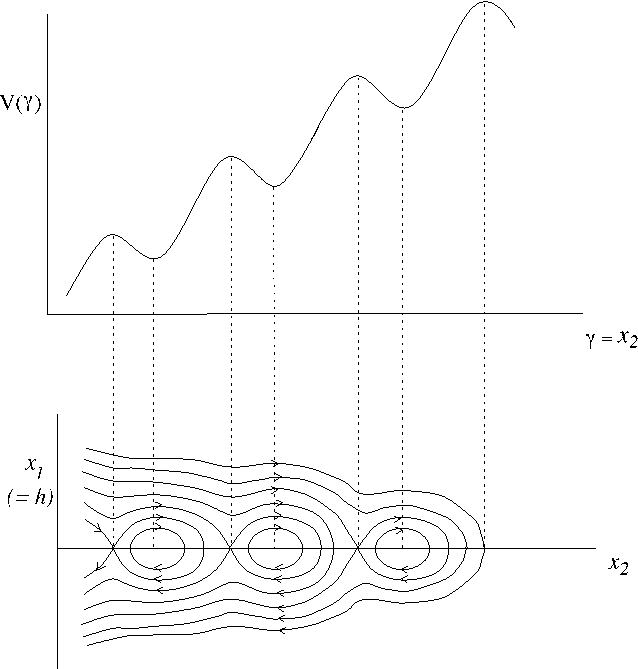
\includegraphics[width=\textwidth*2/3]{figures/asme_portrait}
\end{center}
\caption{Phase portrait}
\label{F:phase2}
\end{figure}
\begin{figure}
\begin{center}
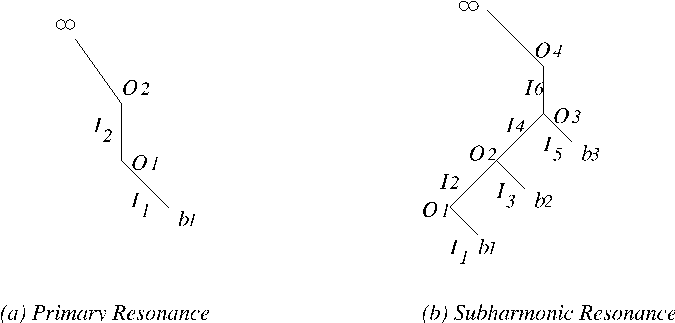
\includegraphics[width=\textwidth]{figures/reducespace}
\end{center}
\caption{Reduced space $\Graph$}
\label{F:reducespace}
\end{figure}

First, the unperturbed averaged Hamiltonian system~\eqref{e:flow} for $m = n = 1$ (i.e., primary resonance) has three fixed points: a center, $b_1$, and two saddles, $\Order_1, \Order_2$ along the $x_2$ ($=\gamma$)-axis. Here the reduced state space is $\Graph = \bigcup_{i=1}^2 \Int_i \bigcup b_1 \bigcup_{i=0}^2 [\Order_i]$, where
\begin{align*}
\Int_1 &\equiv \cup_{\substack{ x=(x_1,x_2) \in \bar \Ss\\
H(x) < \Order_1\\
x \ne b_1}} [x],& \Int_2 &\equiv \cup_{\substack{ x=(x_1,x_2) \in \bar \Ss\\
{\Order}_1<H(x)<{\Order}_2 }} [x],&
\Int_3 &\equiv \cup_{\substack{ x=(x_1,x_2) \in \bar \Ss\\
H(x)>{\Order}_2}}[x].
\end{align*}
See Figure~\ref{F:reducespace}(a). Secondly, the Hamiltonian system~\eqref{e:flow} for $m=3,\ n=1$ (i.e., sub-harmonic resonance) has seven fixed points: three centers, $b_{1,2,3}$, and four saddles, $\Order_{1,2,3,4}$ along the $x_2$-axis. Here the reduced state space is, as illustrated in Figure~\ref{F:reducespace}(b), $\Graph = \bigcup_{i=1}^7 \Int_i \bigcup_{i=1}^3 b_i \bigcup_{i=1}^4 [\Order_i]$, where
\begin{align*}
\Int_1 &\equiv \cup_{\substack{x=(x_1,x_2) \in \bar \Ss\\
H(x)<{\Order}_1\\
x \ne b_1}} [x], & \Int_2 &\equiv \cup_{\substack{ x=(x_1,x_2) \in \bar \Ss\\
{\Order}_1< H(x) < \Order_2\\
x_2 < \{x_2: x = \Order_2 \}}} [x], & \Int_3 &\equiv \cup_{\substack{x=(x_1,x_2) \in \bar \Ss\\
H(x)<{\Order}_2\\
x \ne b_2\\
x_2 > \{x_2: x = \Order_4\}}} [x]\\
\Int_4 &\equiv \cup_{\substack{ x=(x_1,x_2) \in \bar \Ss\\
\Order_2 < H(x) < \Order_3\\
x_2 < \{x_2:x = \Order_3\}}} [x], & \Int_5 &\equiv \cup_{\substack{ x = (x_1,x_2) \in \bar \Ss\\
H(x)<{\Order}_2\\
x \ne b_3\\
x_2 > \{x_2:x = \Order_3\}}} [x], & \Int_6 &\equiv \cup_{\substack{x = (x_1,x_2) \in \bar \Ss\\
{\Order}_3<H(x) < \Order_4}} [x]\\
& &
\Int_7 &\equiv \cup_{\substack{ x=(x_1,x_2) \in \bar \Ss \\
H(x)>{\Order}_4}} [x]
\end{align*}
It should be noted that the Hamiltonian system is $2m\pi$ periodic in the angle variable $x_2$. Namely, the potential for the primary resonance (1:1) contains a single well while the potential for the sub-harmonics (3:1) contains three wells. Besides, except for the orbits inside the closed homoclinic orbits, the remnant of orbits have open trajectories, i.e., their periods become infinite. Henceforth, we can no longer carry out the averaging in the path integrals, namely, the integration with respect to the \emph{Hausdorff measure} in Definition~\ref{D:AVE}. The time averaged drift and diffusion coefficients on each leg $\Int_i$ are calculated as
\begin{align*}
\Tave & (\gen H -(b^1, \nabla K)) =\frac{2m \Omega^\prime (I^{m:n}) \mu_1^2 \left[(1 - k^2) K(k) + (2k^2-1)E(k)\right]}{3\pi n \Omega(I^{m:n}) (1-2k^2)^{3/2}}\\
& - m \Omega^\prime(I^{m:n}) \zeta h^2 \left[(1 - 2k^2)^2 E^2(k)-2(1-3k^2+2k^4)E(k)K(k)+ \right.\\
& \left.(1-5k^2+4k^4)K^2(k) \right]/ \left[3k^2(k^2-1)K^2(k)\right]\\
& + m \Omega^\prime(I^{m:n}) \mu_0 (1 - 2k^2)^2 \pi\ \omega\ \sech^2 A h^2 \sin \gamma \times\\
& \left[-2\cosh A K(k) \left\{(1-2k^2)E(k)+(k^2-1)K(k)\right\} + \right.\\
& \left. \sinh A (2k^2-1)m \pi \left\{ E(1 - k^2)K(k)+(E(k)-K(k))K(1 - k^2)\right\} \right]/\\
& \left[4 \sqrt{2} k^2 \sqrt{1 - 2k^2}(k^2 - 1)K^3(k)\right]\\
& + \frac{m}{4 \pi} (\zeta J_1 -\mu_0 J_2 \Omega^{''}(I^{m:n}) h^2 \sin \gamma)
+ \frac{m}{2 \pi} (\zeta J_1 -\mu_0 J_2 \sin\gamma) \zeta{\mathcal E}_1\\
& +\frac{ (\zeta J_1 -\mu_0 J_2 \sin \gamma)}{2 \pi} \mu_0 (1 - 2k^2)^2 \pi \omega \sech^2 A \cos \gamma \times\\
& \left[- 2\cosh A K(k) \left\{(1-2k^2)E(k)+(k^2-1)K(k)\right\} + \right.\\
& \left. \sinh A (2k^2-1) m \pi \left\{ E(1 - k^2) K(k) + (E(k) - K(k)) K(1 - k^2)\right\} \right]/\\
&\left[ 4\sqrt{2} \ k^2\sqrt{1-2k^2}(k^2-1)K^3(k)\right]
+ \frac{m}{2\pi} \Omega'(I^{m:n})(\zeta J_1-\mu_0 J_2 \sin \gamma) \mathcal E_2,\\
\Tave &(\langle dH, dH \rangle) = \frac{4 m^2 {\Omega'} ^2(I^{m:n}) 
\mu_1^2 h^2 \left[(1-k^2) K(k)+(2k^2-1)E(k)\right]}{3\pi
n\Omega(I^{m:n}) (1-2k^2)^{3/2}}
\end{align*}
where
\begin{gather*}
\begin{aligned}
A &= \frac{m \pi K(1 - k^2)}{2K(k)}, & \mathcal E_1 &= \frac{\omega}{2\pi m}\left.\int_0^{2\pi m/\omega} \frac{\partial x}{\partial I} y \ dt \right|_{I=I^{m:n}},
\end{aligned}\\
{\mathcal E}_2 = \frac{\omega}{2\pi m} \int_0^{2\pi m/\omega}
u_1 ds.
\end{gather*}
Here the modulus $k$ is determined by the resonant orbit $I^{m:n}$ and the detailed calculation of time averaging above are available in \citet[Appendix F]{choi03:_dynam}.

\begin{figure}
\begin{center}
\psfrag{h}{$H$}
\psfrag{b}{$\mathring b$}
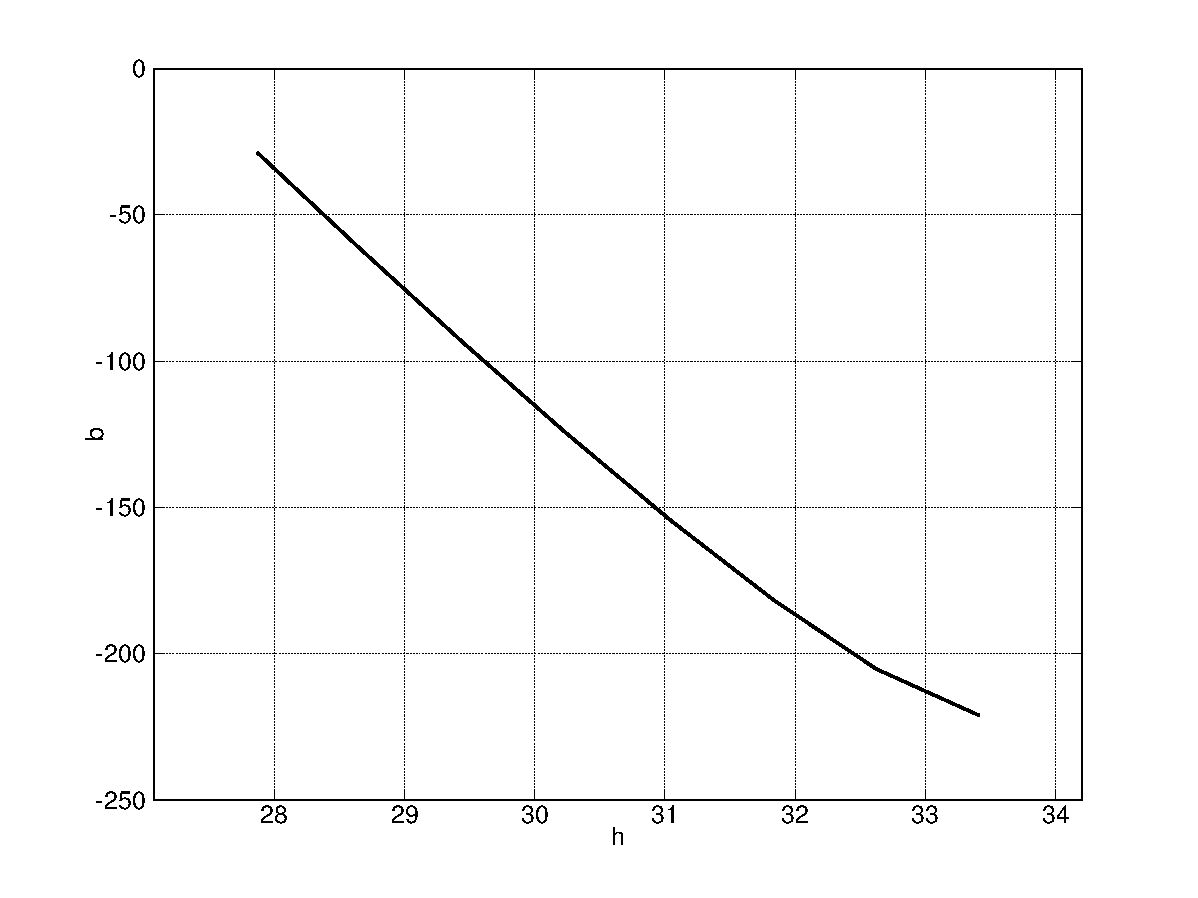
\includegraphics[width=\textwidth*7/8]{figures/oscillator_drift}
\caption{Drift coefficient, $\mathring b$, as a function of the Hamiltonian, $H$.}
\label{f:drift}
\end{center}
\end{figure}

\begin{figure}
\begin{center}
\psfrag{h}{$H$}
\psfrag{s}{$\mathring \sigma$}
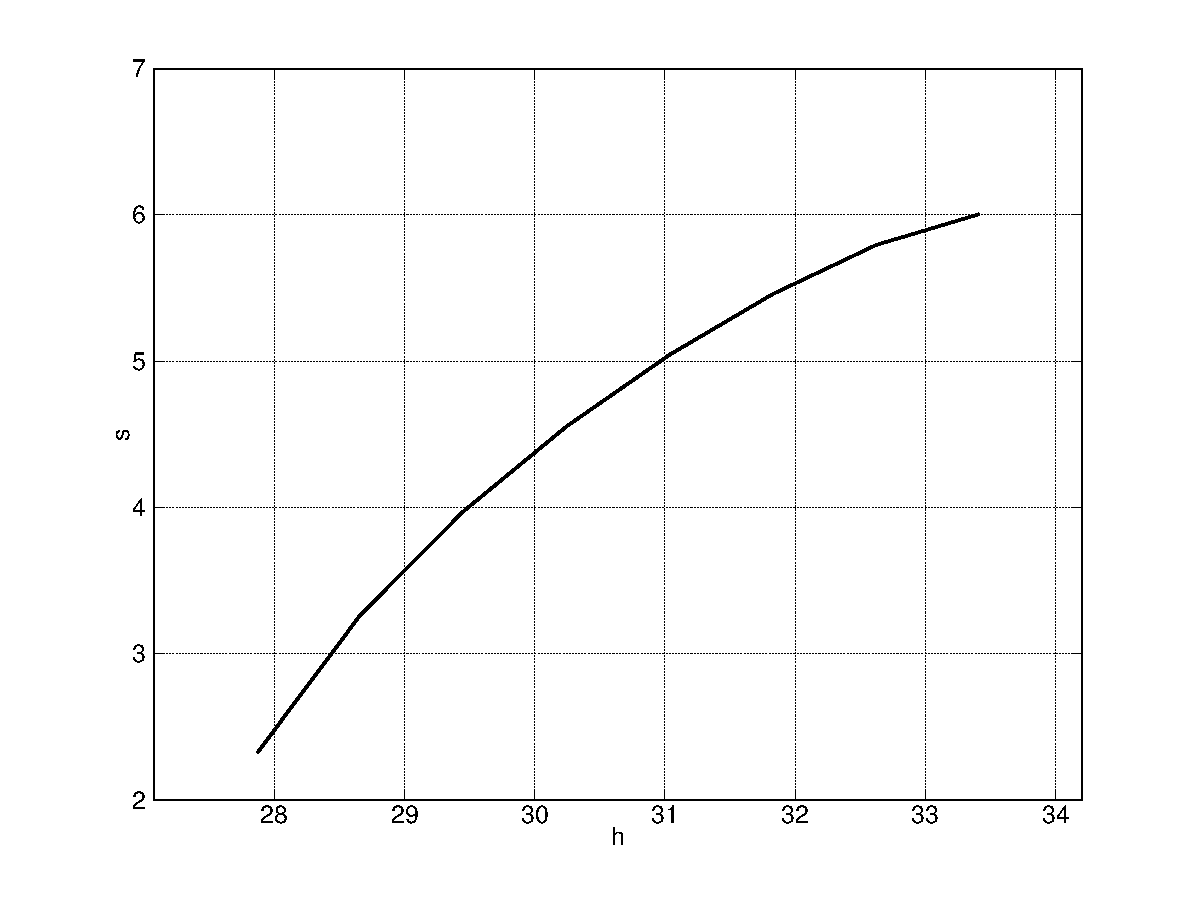
\includegraphics[width=\textwidth*7/8]{figures/oscillator_diffusion}
\caption{Diffusion coefficient, $\mathring \sigma$, as a function of the Hamiltonian, $H$.}
\label{f:diffusion}
\end{center}
\end{figure}

\section{Stationary Probability Density}
\label{S:stationary pdf}

In this section, we examine the stationary probability density of random motions in the resonance zone. The stationary probability density is obtained by solving the Fokker--Planck equation, namely,
\begin{equation}
\gen_i^{adj}\ p_i(z)=-\frac{1}{\period_i}J_i'(z_i) =0, \quad z \in \Int_i,
\label{e:FPE}
\end{equation}
where the probability current which is constant in each leg $\Int_i$ is defined
\[
J_i(z) \equiv \mathring b_i(z) p_i(z)- \frac12
\left({\mathring \sigma}^2_i(z) p_i(z)\right)', \quad z \in
\Int_i,
\]
where the definitions of $\mathring b$ and $\mathring \sigma$ follow Equations \eqref{e:oscillator drift} and \eqref{e:oscillator diffusion}, but the $\Aave$ averaging operator is applied without division by the period.

The limiting domain for our case is
\begin{multline*}
\dom^{adj} = \{p\in C(\Graph)\cap C^2(\cup_{i=1}^N\Int_i):
\text{$\lim_{h \to h_s}(\gen^{adj}_i p_i)(h)$ exists $\forall
i$,}\\
\sum (\pm)J_i(h_s)=0, \text{ and } J_i(\crit_i)=0 \},
\label{E:dom-adjoint}
\end{multline*}
At each of the centers, the so called \emph{entrance boundary} is prescribed because the drift coefficient at the centers is positive whereas the diffusion coefficient is equal to zero. Physically speaking, an entrance boundary (or reflecting boundary) cannot be reached from the interior of the state space because the positive sign of the drift pushes towards the inside. Thus, there is zero net flow of probability across the boundary, which implies that the probability current (or flux) in each leg $\Int_i$ which contains a center becomes identically zero. The reader is referred to \citet{karlin81:_secon_cours_stoch_proces} for a detailed discussion regarding the classification of boundaries. Further, the conservation of probability flux at the interior vertices is imposed

The solution of~\eqref{e:FPE} for the energy level sets is obtained as
\begin{multline*}
p_i(h) = \frac{1}{{\mathring{\sigma}}^2_i(h)}\exp
\left\{2\int^h_{h_i^\crit} \frac{\mathring{b}_i(\eta)}{{\mathring{\sigma}}^2_i(\eta)}\ d\eta \right\} \times\\
\left[ C_i \int^h_{h_i^\crit} \exp \left\{-2
\int^\eta_{h_i^\crit}\frac{\mathring{b}_i(\xi)}{{\mathring{\sigma}}^2_i(\xi)}\
d\xi \right\}\ d\eta +D_i \right] .
\end{multline*}
We need to determine unknown constants $C_i$ and $D_i$ from the prescribed conditions. First, $C_i$'s become identically zero due to the fact of zero probability current condition in the legs $\Int_i$'s which include the centers in Fig.~\ref{F:reducespace}. On the other hand, we have the same constant probability current in the rest of legs due to the conservation of probability current at the interior vertices. We specify the conditions necessary to solve the unknown constants for the primary and sub-harmonic resonance, respectively. For the primary resonance ($1:1$) we encounter $3$ unknown constants, i.e., $D_1,\ C_2,\ D_2$. Then in order to determine them, we apply one continuity and one periodic boundary condition at the saddles
\[
p_1(\Order_1)=p_2(\Order_1)=p_2(\Order_2)
\]
normalization. For the sub-harmonic resonance case ($3:1$), we have
$9$ unknowns, i.e., $D_1,\ C_2,\ D_2,\ D_3,\ C_4,\ D_4,\ D_5,\
C_6,\ D_6$. Thus, in order to determine them completely, we need
nine conditions. Firstly, we apply five continuity conditions and
one periodic boundary condition at the saddle points
\begin{align*}
p_1(\Order_1) &= p_2(\Order_1)=p_6(\Order_4)\\
p_2(\Order_2) &= p_3(\Order_2)=p_4(\Order_2)\\
p_4(\Order_3) &= p_5(\Order_3)=p_6(\Order_3).
\end{align*}
Secondly, we have the conserved probability current at each of saddle points which leads to
\[
C_2 = C_4 = C_6,
\]
and the normalization,
\[
\sum_{i=1}^N \int_{z\in \Int_i} p_i(z)\ dz = 1
\]
completes the determination of the constants.

Graphical results are given in Figures~\ref{reson_den1} and \ref{reson_den2}. For the primary resonance case, we have set the driving frequency $\omega=2$, the damping coefficient $\zeta=1$, the amplitude of the periodic force $\mu_0 = (R^m + 5) \zeta$, and the ratio $R^m(\omega)=3.97$. The corresponding resonant orbit which is determined by the resonance condition becomes $I^{1:1}=0.6345$ in terms of the elliptic modulus. In a similar manner, for the sub-harmonic resonance case, we carried out the numerical analysis with the following values: $\omega=4$, $\zeta=1$, $\mu_0 = (R^m + 20) \zeta$, $R^m(\omega)=23.8$, and $I^{3:1}=0.5068$ (graphical results are omitted.)
\begin{figure}[htbp]
\begin{center}
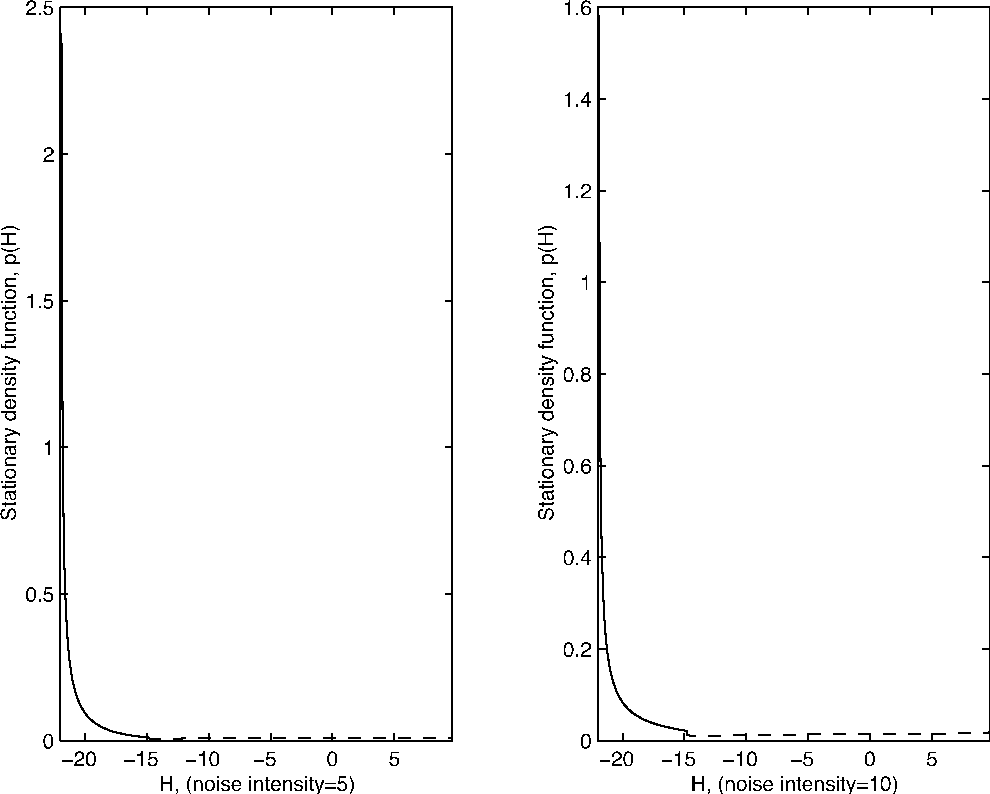
\includegraphics[width=\textwidth]{figures/res_den1}
\caption{Stationary probability density at $1:1$ resonance}
\label{reson_den1}
\end{center}
\end{figure}
\begin{figure}[htbp]
\begin{center}
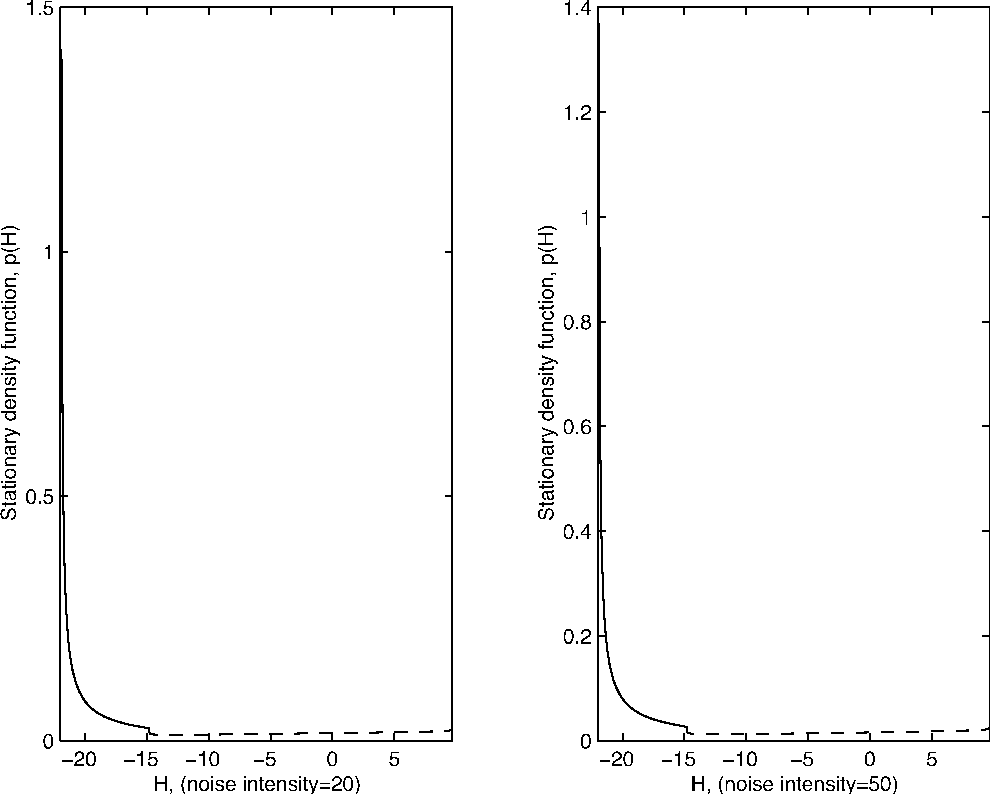
\includegraphics[width=\textwidth]{figures/res_den2}
\caption{Stationary probability density at $1:1$ resonance}
\label{reson_den2}
\end{center}
\end{figure}

\section{Validation With Sample Path Method}

To validate the solutions to the Fokker--Planck equation shown in Figures~\ref{reson_den1} and \ref{reson_den2}, a numerical procedure inspired by the heterogeneous multi-scale methods for stochastic differential equations \citep{e05:_analy} is developed. Instead of solving the FPE, the underlying stochastic differential equations are solved directly.

The stochastic differential equation to be solved is
\begin{equation}
dz = \mathring b(z) dt + \mathring \sigma(z) dW_t,\label{e:hmm sde}
\end{equation}
with $\mathring b$ and $\mathring \sigma$ defined by Equations \eqref{e:oscillator drift} and \eqref{e:oscillator diffusion}. Our numerical validation is used is a multiscale method in the sense that $\Aave$-averaging is performed numerically with time-averaging and the stochastic differential equation above is solved on a longer timescale. At each time-step of the ``macroscopic'' SDE, microscopic $\Aave$-based time averaging is performed.

First, the period of Hamiltonian orbits over which $\Aave$ averaging occurs must be determined. We do this using numerical integration and in that procedure, polar coordinates are used with the arc length being parametrized by the angle variable, $\theta$.

Rewriting the Hamiltonian given in Equation \eqref{E:hamiltonian-ave} as
\[
H = a_1 h^2 + a_2 \gamma + a_3 \cos(\gamma)
\]
where
\begin{align*}
a_1 &= \frac{m}{2} \frac{\partial \Omega}{\partial I} (I^{m:n}), &
a_2 &= \frac{\zeta}{2\pi} J_1, &
a_3 &= \frac{\mu_0}{2\pi} J_2.
\end{align*}
The orbits are translated by $y_c$ so their center is at the origin:
\[
\tilde y = y - y_c,
\]
and polar coordinates are introduced
\begin{align*}
x &= r \cos \theta, &
\tilde y &= r \sin \theta.
\end{align*}
Thus Equation \eqref{E:hamiltonian-ave} becomes
\begin{equation}
H = a_1 (r \cos \theta)^2 + a_2 (r \sin \theta + y_c) + a_3 \cos(r \sin \theta + y_c).
\label{e:hamiltonian polar}
\end{equation}
The arc length formula is
\[
\int_{\theta_1}^{\theta_2} \sqrt{\left(\frac{dr}{d\theta}\right)^2 + r^2} d\theta
\]
Using Equation \eqref{e:hamiltonian polar}, $r(\theta)$ is found numerically (in Octave, the function \emph{fsolve} is used) and to find $dr/d\theta$ one uses
\[
\frac{dr}{d\theta} = \frac{\partial f/\partial \theta}{\partial f/\partial r},
\]
where
\begin{gather*}
\partial f/\partial \theta = -2 a_1 r^2 \cos \theta \sin \theta + a_2 r \cos \theta - a_3 \sin(r \sin \theta + y_c) r \cos \theta,\\
\partial f/\partial r = 2 a_1 r \cos^2 \theta + a_2 \sin \theta - a_3 \sin(r \sin \theta + y_c) \sin \theta.
\end{gather*}
The period is found by numerical quadrature (in Octave, the function \emph{quad} is used.) Thus
\[
T = 2 \int_0^\pi \sqrt{\left(\frac{dr}{d\theta}\right)^2 + r^2} d\theta.
\]

Equation \eqref{e:hmm sde} is solved numerically using the Euler-Maruyama first order scheme \citep{kloeden92:_numer_solut_stoch_differ_equat}
\[
z_{n+1} = z_n + b_n \Delta t + \sigma_n \Xi_{n+1} \sqrt{\Delta t},
\]
where $\Xi_n$ are normally distributed random numbers with mean zero and variance one. Illustrative results obtained with the drift and diffusion coefficients in Figures \ref{f:drift} and \ref{f:diffusion} are shown in Figure \ref{f:sample pdf}.

\begin{figure}
\begin{center}
\psfrag{H}{$H$}
\psfrag{p}{$p$}
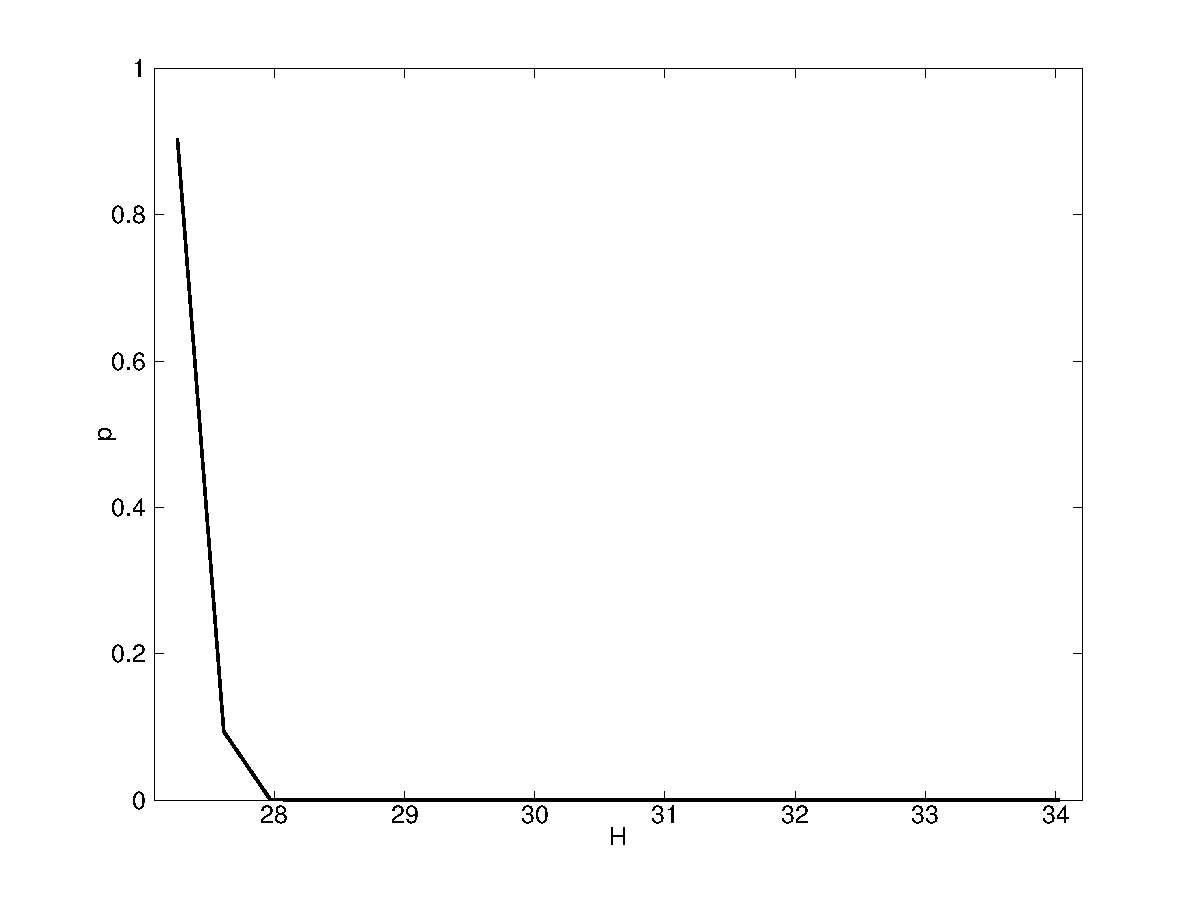
\includegraphics[width=\textwidth*7/8]{figures/oscillator_steady_state_pdf}
\caption{Steady state PDF as a function of the Hamiltonian, $H$. The PDF is produced with the sample path method. 3444 samples have been used. The time-step was set to $10^{-2}$ and 20 time-steps were taken.}
\label{f:sample pdf}
\end{center}
\end{figure}

\section{Conclusions}

An averaging approach has been developed to explore the near resonant motion of a noisy, strongly nonlinear periodically forced system. We first rewrote the perturbed Hamiltonian system with strong nonlinearity in action space by means of a canonical transformation. We introduced local coordinates adjacent to the resonance surface and performed the appropriate rescaling which allows us to see the correct asymptotics. After stochastic averaging, the resulting reduced model became a graph valued process under capture into resonance. Since we addressed a separation of time scales, such a methodology enabled us to diminish the dimension of the original model. The reduced process converged in probability to a Markov process as $\tilde\epsilon \to 0$. The associated limiting generator has furnished statistical quantities such as the probability density function. The effects of noisy perturbations were investigated through such a statistical description.

Some investigators, including \citet{soskin89:_fluct, soskin92:_evolut}, have shown there is no dramatic stochastic resonance phenomenon in a system whose oscillation frequency is a monotonically increasing function of energy (see Fig.~\ref{F:frequency}(a).) In systems with \emph{asymmetric} single-well potentials with a non-monotonic frequency variation (see Fig.~\ref{F:frequency}(b)), however, dramatic stochastic resonance has been shown to emerge at optimal noise. Thus, in view of our analysis, we conjecture that the existence of P-bifurcations in asymmetric systems may be connected to stochastic resonance.
